\documentclass[a4paper,twoside]{article}
\usepackage{blindtext}  
\usepackage{geometry}

% Chinese support
\usepackage[UTF8, scheme = plain]{ctex}

% Page margin layout
\geometry{left=2.3cm,right=2cm,top=2.5cm,bottom=2.0cm}


\usepackage{listings}
\usepackage{xcolor}
\usepackage{geometry}
\usepackage{amsmath}
\usepackage{float}
\usepackage{hyperref}

\usepackage{graphics}
\usepackage{graphicx}
\usepackage{subfigure}
\usepackage{epsfig}
\usepackage{float}

\usepackage{algorithm}
\usepackage[noend]{algpseudocode}

\usepackage{booktabs}
\usepackage{threeparttable}
\usepackage{longtable}
\usepackage{tikz}
\usepackage{multicol}

% cite package, to clean up citations in the main text. Do not remove.
\usepackage{cite}

\usepackage{color,xcolor}

%% The amssymb package provides various useful mathematical symbols
\usepackage{amssymb}
%% The amsthm package provides extended theorem environments
\usepackage{amsthm}
\usepackage{amsfonts}
\usepackage{enumerate}
\usepackage{enumitem}
\usepackage{listings}
\usepackage{minted}


\usepackage{indentfirst}
\setlength{\parindent}{2em} % Make two letter space in the first paragraph
\usepackage{setspace}
\linespread{1.5} % Line spacing setting
\usepackage{siunitx}
\setlength{\parskip}{0.5em} % Paragraph spacing setting

% \usepackage[contents =22920202204622, scale = 10, color = black, angle = 50, opacity = .10]{background}

\renewcommand{\figurename}{图}
\renewcommand{\listingscaption}{代码}
\renewcommand{\tablename}{表格}
\renewcommand{\contentsname}{目录}
\floatname{algorithm}{算法}

\graphicspath{ {images/} }

%%%%%%%%%%%%%
\newcommand{\StudentNumber}{22920202204622}  % Fill your student number here
\newcommand{\StudentName}{熊恪峥}  % Replace your name here
\newcommand{\PaperTitle}{实验(一)MIPS指令系统和MIPS体系结构}  % Change your paper title here
\newcommand{\PaperType}{计算机系统结构实验} % Replace the type of your report here
\newcommand{\Date}{2023年3月8日}
\newcommand{\College}{信息学院}
\newcommand{\CourseName}{计算机系统结构}
%%%%%%%%%%%%%

%% Page header and footer setting
\usepackage{fancyhdr}
\usepackage{lastpage}
\pagestyle{fancy}
\fancyhf{}
% This requires the document to be twoside
\fancyhead[LO]{\texttt{\StudentName }}
\fancyhead[LE]{\texttt{\StudentNumber}}
\fancyhead[C]{\texttt{\PaperTitle }}
\fancyhead[R]{\texttt{第{\thepage}页,共\pageref*{LastPage}页}}


\title{\PaperTitle}
\author{\StudentName}
\date{\Date}

\algnewcommand\algorithmicinput{\textbf{Input:}}
\algnewcommand\algorithmicoutput{\textbf{Output:}}
\algnewcommand\Input{\item[\algorithmicinput]}%
\algnewcommand\Output{\item[\algorithmicoutput]}%

\usetikzlibrary{positioning, shapes.geometric}

\begin{document}
	
%%%%%%%%%%%%%%%%%%%%%%%%%%%%%%%%%%%%%%%%%%%%
\makeatletter % change default title style
\renewcommand*\maketitle{%
	\begin{center} 
		\bfseries  % title 
		{\LARGE \@title \par}  % LARGE typesetting
		\vskip 1em  %  margin 1em
		{\global\let\author\@empty}  % no author information
		{\global\let\date\@empty}  % no date
		\thispagestyle{empty}   %  empty page style
	\end{center}%
	\setcounter{footnote}{0}%
}
\makeatother
%%%%%%%%%%%%%%%%%%%%%%%%%%%%%%%%%%%%%%%%%%%%
	
	
\thispagestyle{empty}

\vspace*{1cm}

\begin{figure}[htb]
	\centering
	
\includegraphics[width=4.0cm]{logo.png}
\end{figure}

\vspace*{1cm}

\begin{center}
	\Huge{\textbf{\PaperType}}
	
	\Large{\PaperTitle}
\end{center}

\vspace*{1cm}

\begin{table}[H]
	\centering	
	\begin{Large}
		\renewcommand{\arraystretch}{1.5}
		\begin{tabular}{p{3cm} p{5cm}<{\centering}}
			姓\qquad 名 & \StudentName  \\
			\hline
			学\qquad号 & \StudentNumber \\
			\hline
			日\qquad期 & \Date  \\
			\hline
			学\qquad院 & \College  \\
			\hline
			课程名称 & \CourseName  \\
			\hline
		\end{tabular}
	\end{Large}
\end{table}

\newpage

\title{
	\Large{\textcolor{black}{\PaperTitle}}
}
	
	
\maketitle
	
\tableofcontents
 
\newpage
\setcounter{page}{1}

\begin{spacing}{1.2}

\section{实验目的}

\begin{enumerate}
	\item 了解和熟悉指令级模拟器
	\item 熟练掌握MIPSsim模拟器的操作和使用方法
	\item 熟悉MIPS指令系统及其特点,加深对MIPS指令操作语义的理解
	\item 熟悉MIPS体系结构
\end{enumerate}

\section{实现阶乘}

\subsection{实现思路}

实现阶乘可以使用循环的方法,使用寄存器\texttt{r2}作为结果,使用寄存器\texttt{r3}
循环计数,循环将\texttt{r2}与\texttt{r3}相乘,然后将结果存入\texttt{r2}中,然后
递减\texttt{r3},直到\texttt{r3}为1,循环结束后,\texttt{r2}中的值即为阶乘的结果。

具体实现如代码~\ref{code:fact}。
\begin{listing}[htb]
	\caption{阶乘代码}
	\label{code:fact}
	\inputminted{nasm}{code/fact.txt}
\end{listing}

运行结果如图~\ref{fig:fact},使用$X=5$进行计算,结果存储在\texttt{R2}中,为$120$。
可见程序是正确的。
\begin{figure}[htb]
	\centering
	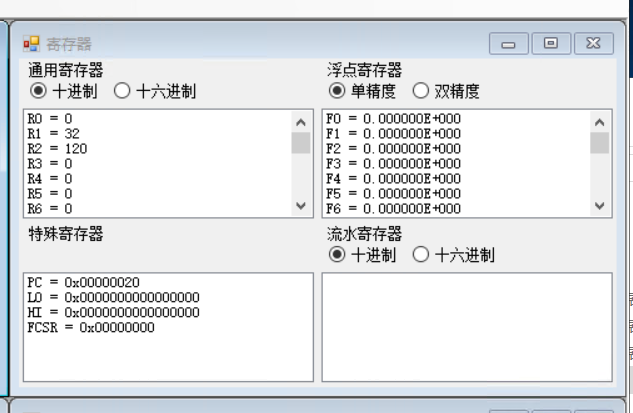
\includegraphics[width=0.4\textwidth]{images/fact.png}
	\caption{阶乘运行结果}
	\label{fig:fact}
\end{figure}

\section{计算$(X-Y) \times 2 - (X+Y)\div 8$}

\subsection{实现思路}

题目要求不使用乘除指令。观察题目要求,可以发现2和8都是2的幂,因此可以使用移位
指令代替乘除指令。具体实现如代码~\ref{code:mul}。
\begin{listing}[htb]
	\caption{计算代码}
	\label{code:mul}
	\inputminted{nasm}{code/mul.txt}
\end{listing}

运行结果如图~\ref{fig:mul},使用$X=5,Y=3$进行计算,结果存储在\texttt{R6}中,为$3$。
可见程序是正确的。
\begin{figure}[ht]
	\centering
	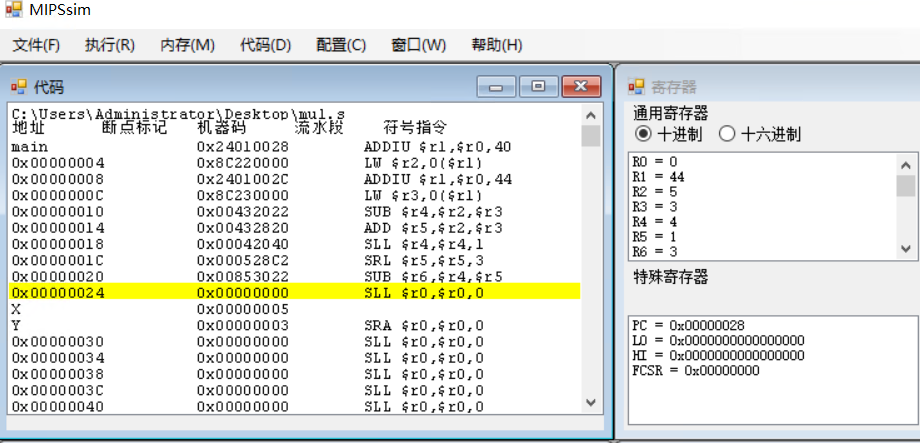
\includegraphics[width=0.8\textwidth]{images/mul.png}
	\caption{计算结果}
	\label{fig:mul}
\end{figure}


\section{写入内存}

\subsection{实现思路}

为了实现将计算结果写入内存,需要使用\texttt{SW}指令将寄存器中的值写入内存中。
具体实现如代码~\ref{code:minus}。
\begin{listing}[htb]
	\caption{计算并写入内存}
	\label{code:minus}
	\inputminted{nasm}{code/minus.txt}
\end{listing}

运行结果如图~\ref{fig:minus},内存单元N中的值初始化为5,程序执行完成后变成4。
\begin{figure}[ht]
	\centering
	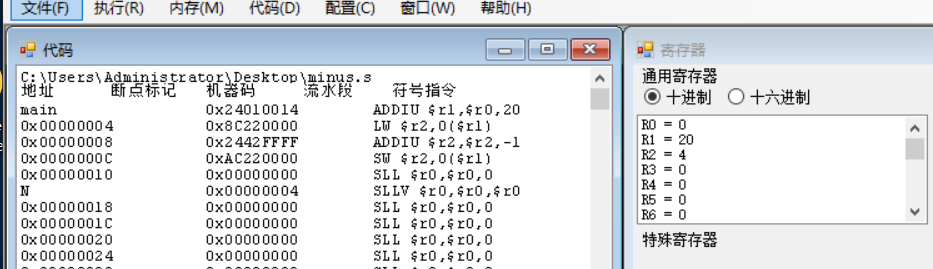
\includegraphics[width=0.8\textwidth]{images/minus.png}
	\caption{计算并写入内存}
	\label{fig:minus}
\end{figure}

\section{实验总结}

本次实验在\texttt{MIPSSim}模拟器中实现了阶乘、计算、写入内存的程序。MIPS是一种
精简指令集。在使用过程中许多操作都与x86汇编有所区别,例如:
\begin{enumerate}
	\item 有较多的寄存器,寄存器的编号与x86不同。
	\item \texttt{MOV}指令与x86不同,功能较为单一
	\item 有较多的三操作数指令
\end{enumerate}
在实验过程中,我初步认识了使用RISC指令集编程的过程,掌握了模拟器的使用和操作。

\end{spacing}

\end{document}